% docx2tex 1.8 --- ``Who let the docx out?'' 
% 
% docx2tex is Open Source and  
% you can download it on GitHub: 
% https://github.com/transpect/docx2tex 
%  
\documentclass[11pt]{article}
\usepackage[a4paper,total={6in,8in},margin=1in]{geometry}
\usepackage[utf8]{inputenc} % allow utf-8 input
\usepackage[T1]{fontenc}    % use 8-bit T1 fonts
\usepackage{microtype,inconsolata}
\usepackage{times,latexsym}
\usepackage{graphicx} \graphicspath{{figures/}}
\usepackage{amsmath,amssymb,mathabx,mathtools,amsthm,nicefrac}
\usepackage[linesnumbered,ruled,vlined]{algorithm2e}
\usepackage{enumitem}
\usepackage[pagebackref,breaklinks,colorlinks]{hyperref}
\usepackage[skip=3pt,font=small]{subcaption}
\usepackage[skip=3pt,font=small]{caption}
\usepackage[dvipsnames,svgnames,x11names,table]{xcolor}
\usepackage[capitalise,noabbrev,nameinlink]{cleveref}
\usepackage{booktabs,tabularx,colortbl,multirow,multicol,array,makecell,tabularray}
\usepackage[english]{babel}
\definecolor{color-C00000}{rgb}{0.75,0,0}
\definecolor{red}{rgb}{1,0,0}

\begin{document}
{\centering \textbf{CV1 : project \#2 } (total 10 points)

\par}{\centering \textbf{Restoration and Inpainting} \par}
{\centering Due October 26th (Thur), 2023, 11:59pm

\par}   

\section{Background} 

This project is based on Section 3.2.1, Section 3.2.2, and Section 3.2.3 of the textbook. You shall read the corresponding parts and understand the underlying logistics before writing your code.

\subsection{Python Library}
Please install the latest cv2, PIL, numpy, scipy, matplotlib, tqdm, torch (including torch-vision), and the cython (if you want) packages. You are also welcome to utilize any libraries of your choice, \textbf{but please report them in your report (for autograder)!}
\color{red}
\textbf{Again, report any customized library in the report (do not go too crazy as this will add a significant burden to TAs).}
\color{black}



\subsection{What to hand in?}

Please submit both a formal report and the accompanying code. For the report, kindly provide a PDF version. You may opt to compose a new report or complete the designated sections within this document, as can be started by simply loading the tex file to Overleaf. Your score will be based on the quality of \textbf{your results}, \textbf{the analysis} (diagnostics of issues and comparisons) of these results in your report, and your \textbf{code implementation}.

\paragraph{Notice}

\begin{enumerate}
    \item There is no immediate feedback autograder to help with the debugging this time. The autograder will be run after the end of the homework!
    \item Do not modify the function names in the given code, unless explicitly specified in this document.
\end{enumerate}


\subsection{Help}

Make a diligent effort to independently address any encountered issues, and in cases where challenges exceed your capabilities, do not hesitate to seek assistance! Collaboration with your peers is permitted, but it is crucial that you refrain from directly \textcolor{red}{examining or copying one another's code.}  Please be aware that you'll fail the course if our \textbf{code similarity checker}, which has found some prohibited behaviors for Project 1, detects these violations.

For details, please refer to \url{https://yzhu.io/s/teaching/plagiarism/}

\clearpage

\section{Objective}

This project serves as a preliminary exercise so that you can get familiar with Gibbs/MRF models, the fundamental principles of the Gibbs sampler, and the application of Partial Differential Equations (PDE) in the context of image restoration and inpainting. Three kinds of images are featured in the illustration presented below, all enclosed within the compressed file provided. The original image comprises distinct color bands, specifically Red, Green, and Blue. At the same time, the distorted counterpart is the result of superimposing a mask image onto the \textbf{Red band} of the original image. It is worth noting that two image sets are provided, one featuring a small font size, and the other, a big font size.
\begin{figure}[ht!]
    \centering
    \hfill%
    \begin{subfigure}[]{0.333\linewidth}
        \centering
        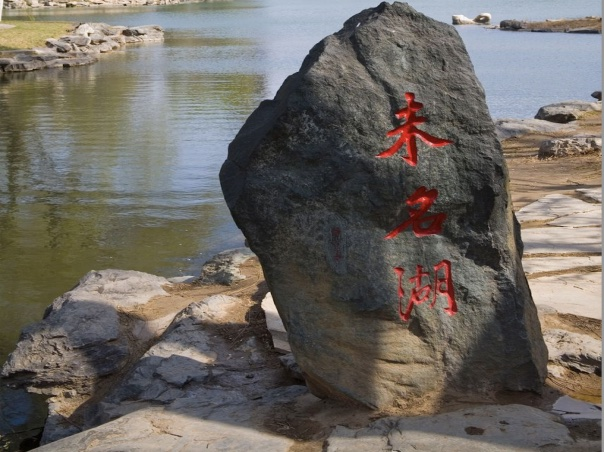
\includegraphics[width=\linewidth]{fig/stone_ori.jpg}
        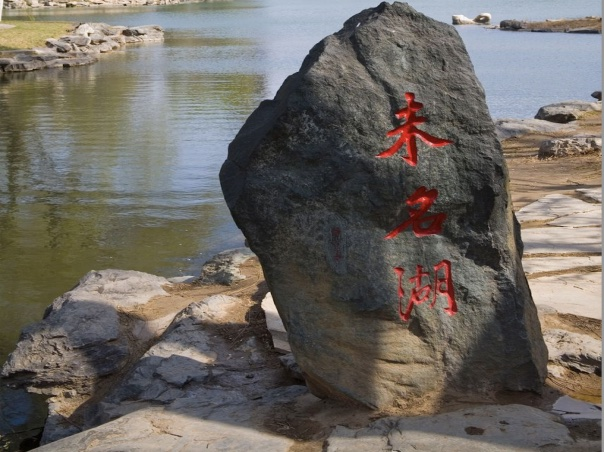
\includegraphics[width=\linewidth]{fig/stone_ori.jpg}
        \caption{Original Image}
    \end{subfigure}%
    \hfill%
    \begin{subfigure}[]{0.333\linewidth}
        \centering
        
\includegraphics[width=\linewidth]{fig/mask_big.jpg}
        
\includegraphics[width=\linewidth]{fig/mask_small.jpg}
        \caption{Mask Image}
    \end{subfigure}%
    \hfill%
    \begin{subfigure}[]{0.333\linewidth}
        \centering
        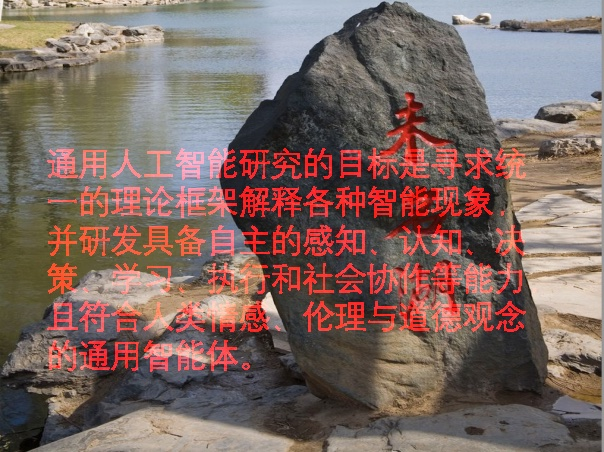
\includegraphics[width=\linewidth]{fig/imposed_stone_big.jpg}
        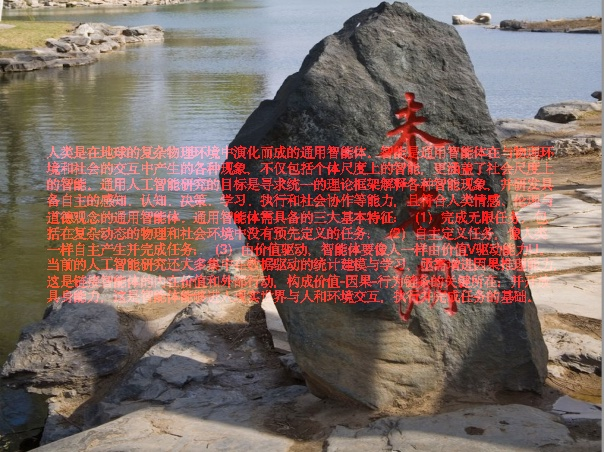
\includegraphics[width=\linewidth]{fig/imposed_stone_small.jpg}
        \caption{Distorted Image}
    \end{subfigure}%
\end{figure}


 In this experimental setting, pretend that you are provided solely with the distorted image denoted as \textbf{I} in subfigure (c) and the corresponding mask image \textbf{M} featured in subfigure (b). The primary objective of this experiment is to reconstruct the original image, represented as \textbf{O}, by filling in the masked pixels exclusively within the Red-band. It is essential to underscore that no restorative action is required for the Green and Blue bands. Given that information within the masked pixels has been irreversibly compromised, our task is to approximate the original image as \textbf{X}, which serves as an estimable substitute for \textbf{O}. To evaluate the efficacy of this restoration process, a per-pixel error assessment must be undertaken, explicitly concerning all the pixels concealed by the mask, comparing the reconstructed \textbf{X} with the ground truth image \textbf{O}.

 As demonstrated below, to make the project more interesting, we offer three original images, and their corresponding distorted version. Note that all of the images are of the same size, and they are masked at the same place. \textbf{You should conduct experiments on all of them.}
 \begin{figure}[ht!]
    \centering
    \hfill%
    \begin{subfigure}[]{0.333\linewidth}
        \centering
        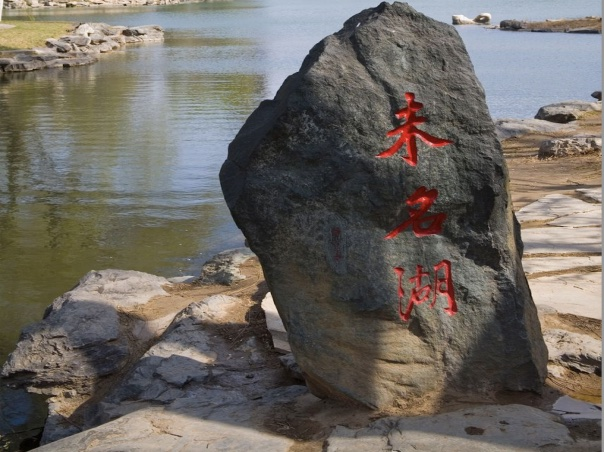
\includegraphics[width=\linewidth]{fig/stone_ori.jpg}
        \caption{stone}
    \end{subfigure}%
    \hfill%
    \begin{subfigure}[]{0.333\linewidth}
        \centering
        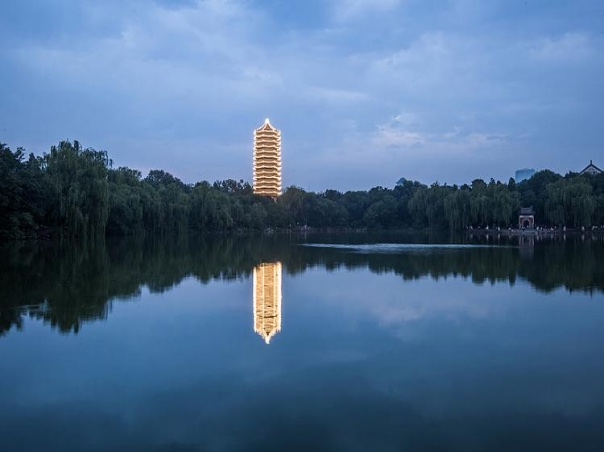
\includegraphics[width=\linewidth]{fig/sce_ori.jpg}
        \caption{sce}
    \end{subfigure}%
    \hfill%
    \begin{subfigure}[]{0.333\linewidth}
        \centering
        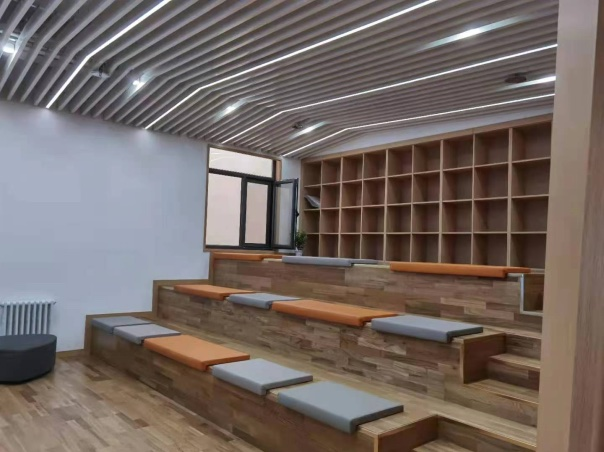
\includegraphics[width=\linewidth]{fig/room_ori.jpg}
        \caption{room}
    \end{subfigure}%
\end{figure}

\clearpage

\section{Method 1: Gibbs Sampler}

\subsection{Overview}

 Let $\Lambda $ be the white pixels in the mask image \textbf{M} (distorted in I), and $\partial \Lambda $ the boundary condition (i.e., the undistorted pixels), which will stay unchanged. We compute
\begin{equation*}
  X_{\Lambda }| X_{\partial \Lambda } \sim  p(X_{\Lambda }|X_{\partial \Lambda })
\end{equation*}
by sampling from a Gibbs or MRF model of the following form
\begin{equation*}
p(X_{\Lambda }|X_{\partial \Lambda })=\frac{1}{Z} \exp\{ -\beta \sum _{(x,y)\in \Lambda } E(\nabla _{x} X(x,y))+ E(\nabla _{y}X(x,y)) \},
\end{equation*}
where E() is a potential energy. We need to try two choices of functions:\begin{itemize}
    \item $L_1$ norm: $E( \nabla_x X(x,y)) = |\nabla_x X(x,y)|$
    \item $L_2$ norm: $E( \nabla_x X(x,y)) = (\nabla_x X(x,y))^2$.
\end{itemize}
From this Gibbs model, we can derive the local characteristics, given
\begin{equation*}
    X_s \sim p(X_s|X_{\partial s}), \forall s \in \Lambda.
\end{equation*}
By drawing from this 1D probability (using the inverse CDF method mentioned in Project 1), we can iteratively compute the values of the distorted pixels. Visiting all distorted pixels once is called 1-sweep (in whatever order, it does not matter). You need to experiment with an annealing scheme by slowly increasing the parameter $\beta $ from 0.1 to 1 (or more).

\subsection{Instructions}

\begin{enumerate}
    \item Please read through the main file and understand the whole logic.
    \item Please implement the ``conv()'' function, which calculates the x direction and y direction gradients. Please be careful that the function's return should hold the same shape as the input, and the boundary condition selected is \textbf{periodic boundary condition}.    
    \item Please implement the ``gibbs\_sampler()'' function designed to execute Gibbs sampling for an individual pixel. (Hints: Consider optimizations to enhance computational efficiency by avoiding superfluous calculations.)
    \item Implement the main function and tune the parameters for better effect.
\end{enumerate}

\section{Method 2: PDE}

\subsection{Overview}

 For $L_2$-norm energy functions, you can minimize the energy by the heat-diffusion equation. 
 \subsection{Instructions}
 \begin{enumerate}
     \item Implement the ``pde()'' function, which performs pde update for a specific pixel. 
     \item Implement the main function and tune the parameters for better effect. 
     \item Please run more sweeps to see the marvelous effect of this method.
 \end{enumerate}
 
\section{Speed Up (Optional)}

This is not required in this project, and there is no extra bonus for implementing it. If you have time, you can have a try.
\begin{enumerate}
    \item If your implementation is done by using Torch, it'll be much faster to change to numpy.
    \item Use the \textbf{cython} library! Please first read the \href{https://cython.readthedocs.io/en/latest/src/tutorial/cython_tutorial.html}{basic tutorial}, and understand some basic logistics of \textbf{cython}. Please be cautious that the \textbf{``pyximport'' method} is the \textbf{preferred approach} as opposed to the \textbf{``setup.py'' method}. The latter may generate different files on different operating systems, and it's important to be aware that the autograder utilizes the Linux operating system. Now, you are almost ready to speed up your Gibbs sampling, please read the \href{https://cython.readthedocs.io/en/latest/src/tutorial/numpy.html}{working with numpy} section of the document. You have done a great job, and please speed up your Gibbs sampling process with Cython!
\end{enumerate}

\section{Hand-in}

\begin{enumerate}
    \item Plot the per pixel error $\frac{1}{|\Lambda|} \sum (X(x,y) -  O(x,y)) ^ 2$ over the number of sweeps t in for both methods. 
    \item Show the restored image sequence corresponding to the number of sweeps.
    \item \textbf{(Bonus, Optional)} Where are the original images from? Try to find them in PKU, take nice photos of them at a similar angle, report their names, and submit your photos. 
\end{enumerate}

\section{Results}

\subsection{Per Pixel Error}

\subsubsection{Gibss Restoration}

\begin{figure}[ht!]
    \centering
    \hfill%
    \begin{subfigure}[]{0.333\linewidth}
        \centering
        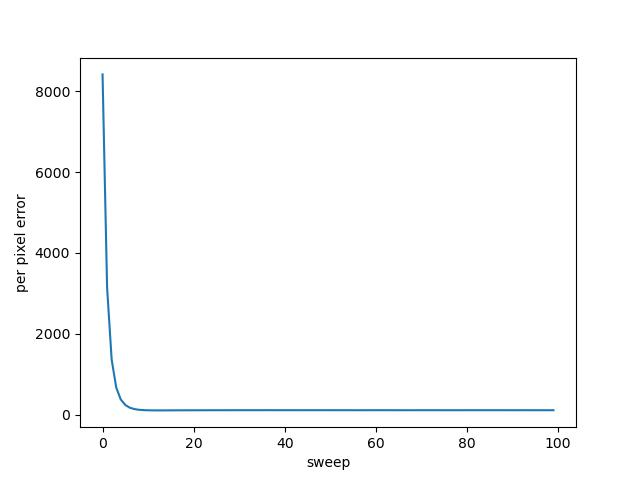
\includegraphics[width=\linewidth]{fig/loss/stone_L1_small_loss.jpg}
        \caption{stone L1 small}
    \end{subfigure}%
    \hfill%
    \begin{subfigure}[]{0.333\linewidth}
        \centering
        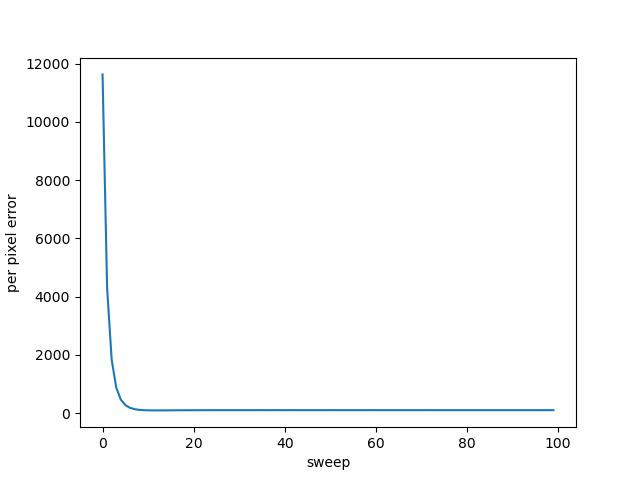
\includegraphics[width=\linewidth]{fig/loss/sce_L1_small_loss.jpg}
        \caption{sce L1 small}
    \end{subfigure}%
    \hfill%
    \begin{subfigure}[]{0.333\linewidth}
        \centering
        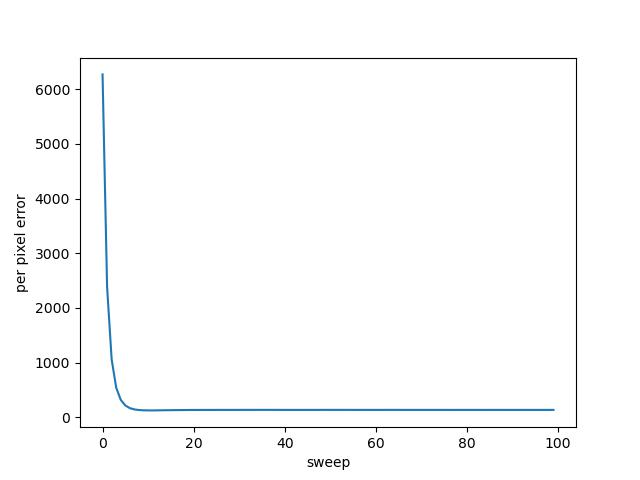
\includegraphics[width=\linewidth]{fig/loss/room_L1_small_loss.jpg}
        \caption{room L1 small}
    \end{subfigure}%
\end{figure}

\begin{figure}[ht!]
    \centering
    \hfill%
    \begin{subfigure}[]{0.333\linewidth}
        \centering
        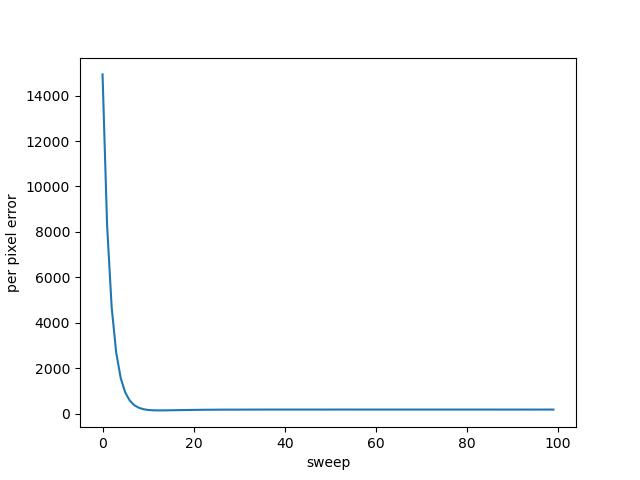
\includegraphics[width=\linewidth]{fig/loss/stone_L1_big_loss.jpg}
        \caption{stone L1 big}
    \end{subfigure}%
    \hfill%
    \begin{subfigure}[]{0.333\linewidth}
        \centering
        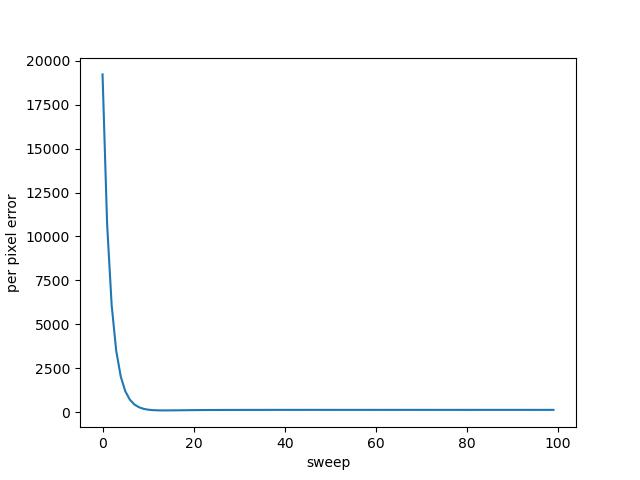
\includegraphics[width=\linewidth]{fig/loss/sce_L1_big_loss.jpg}
        \caption{sce L1 big}
    \end{subfigure}%
    \hfill%
    \begin{subfigure}[]{0.333\linewidth}
        \centering
        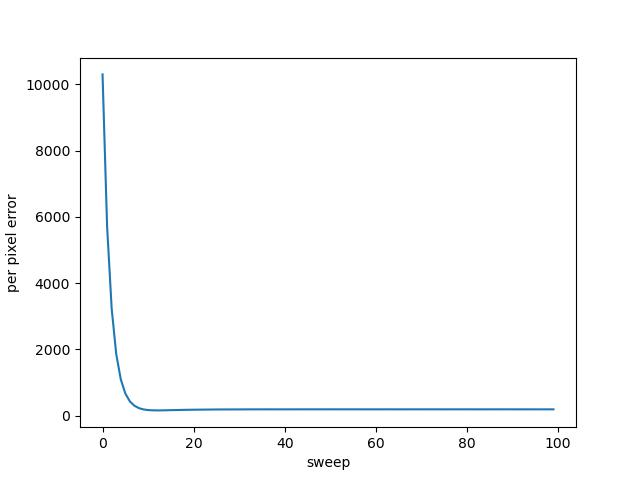
\includegraphics[width=\linewidth]{fig/loss/room_L1_big_loss.jpg}
        \caption{room L1 big}
    \end{subfigure}%
\end{figure}

\begin{figure}[ht!]
    \centering
    \hfill%
    \begin{subfigure}[]{0.333\linewidth}
        \centering
        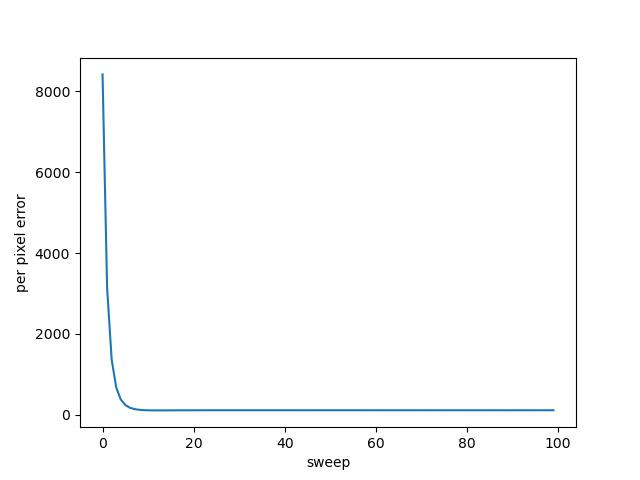
\includegraphics[width=\linewidth]{fig/loss/stone_L2_small_loss.jpg}
        \caption{stone L2 small}
    \end{subfigure}%
    \hfill%
    \begin{subfigure}[]{0.333\linewidth}
        \centering
        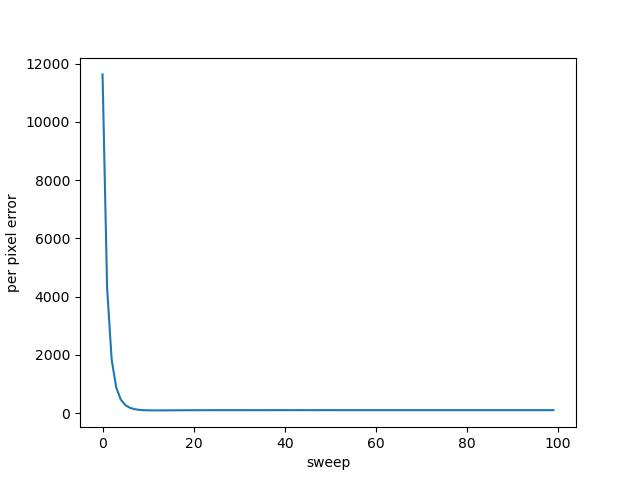
\includegraphics[width=\linewidth]{fig/loss/sce_L2_small_loss.jpg}
        \caption{sce L2 small}
    \end{subfigure}%
    \hfill%
    \begin{subfigure}[]{0.333\linewidth}
        \centering
        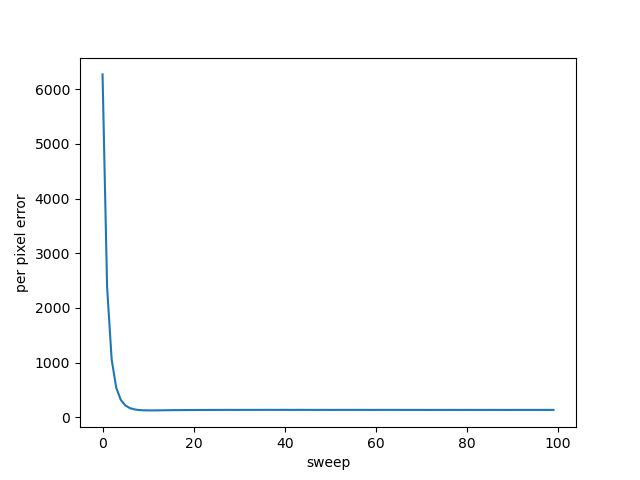
\includegraphics[width=\linewidth]{fig/loss/room_L2_small_loss.jpg}
        \caption{room L2 small}
    \end{subfigure}%
\end{figure}

\begin{figure}[ht!]
    \centering
    \hfill%
    \begin{subfigure}[]{0.333\linewidth}
        \centering
        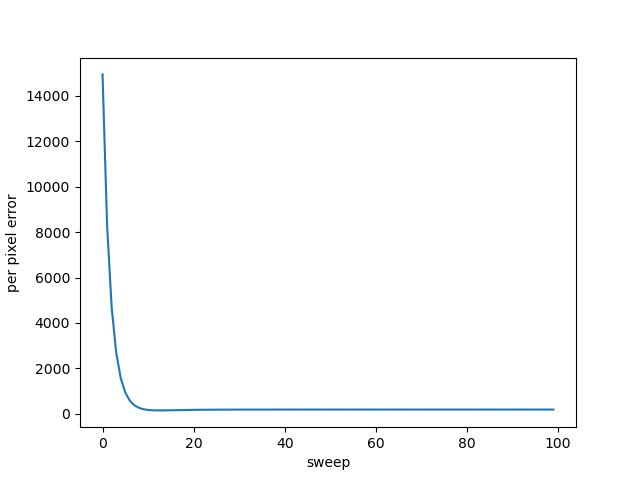
\includegraphics[width=\linewidth]{fig/loss/stone_L2_big_loss.jpg}
        \caption{stone L2 big}
    \end{subfigure}%
    \hfill%
    \begin{subfigure}[]{0.333\linewidth}
        \centering
        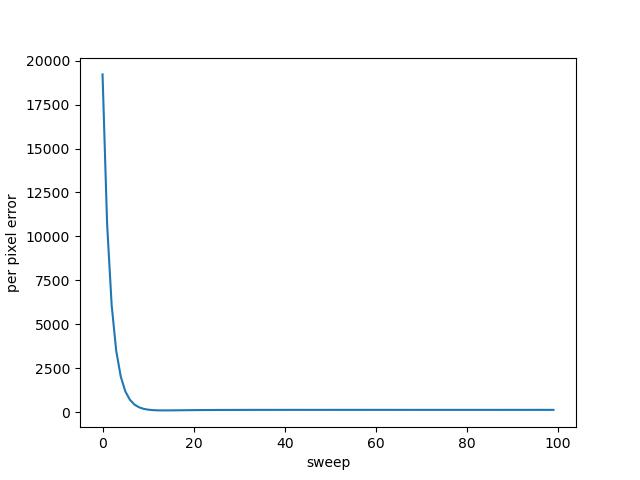
\includegraphics[width=\linewidth]{fig/loss/sce_L2_big_loss.jpg}
        \caption{sce L2 big}
    \end{subfigure}%
    \hfill%
    \begin{subfigure}[]{0.333\linewidth}
        \centering
        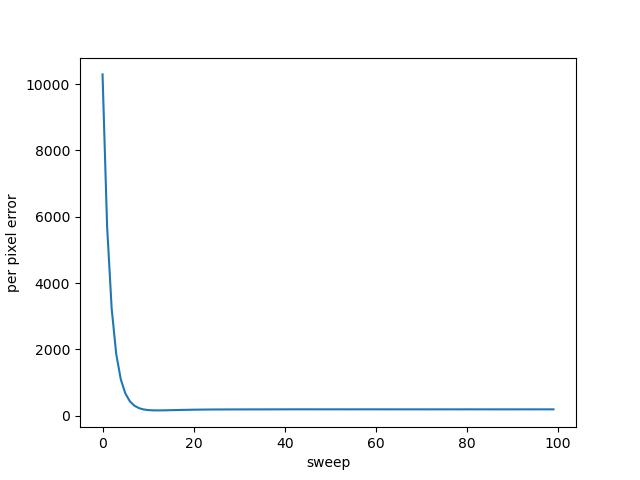
\includegraphics[width=\linewidth]{fig/loss/room_L2_big_loss.jpg}
        \caption{room L2 big}
    \end{subfigure}%
\end{figure}

\subsubsection{PDE Restoration}

\begin{figure}[ht!]
    \centering
    \hfill%
    \begin{subfigure}[]{0.333\linewidth}
        \centering
        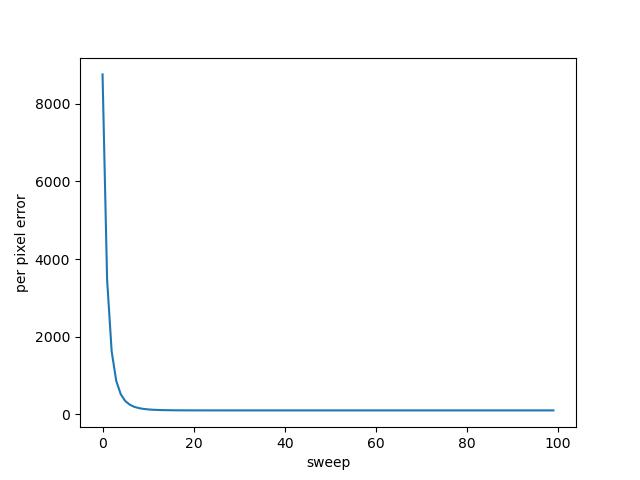
\includegraphics[width=\linewidth]{fig/loss/stone_small_loss.jpg}
        \caption{stone small}
    \end{subfigure}%
    \hfill%
    \begin{subfigure}[]{0.333\linewidth}
        \centering
        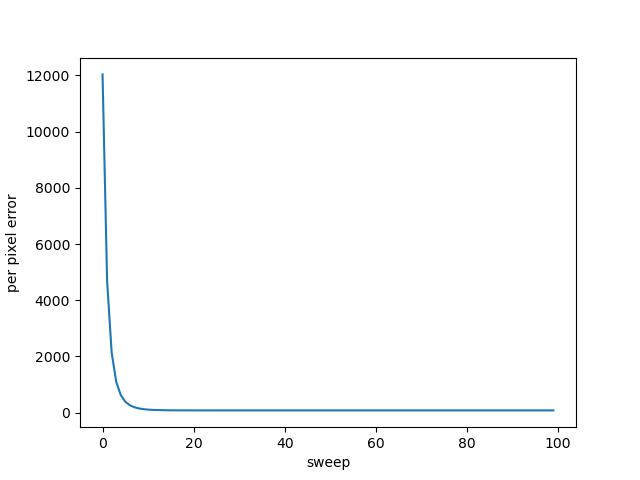
\includegraphics[width=\linewidth]{fig/loss/sce_small_loss.jpg}
        \caption{sce small}
    \end{subfigure}%
    \hfill%
    \begin{subfigure}[]{0.333\linewidth}
        \centering
        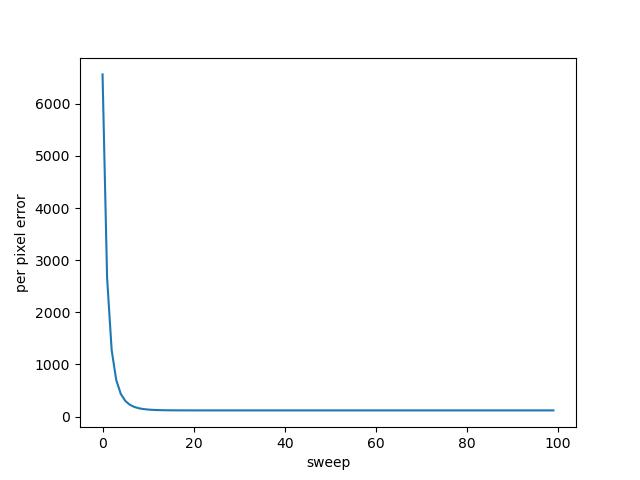
\includegraphics[width=\linewidth]{fig/loss/room_small_loss.jpg}
        \caption{room small}
    \end{subfigure}%
\end{figure}

\begin{figure}[ht!]
    \centering
    \hfill%
    \begin{subfigure}[]{0.333\linewidth}
        \centering
        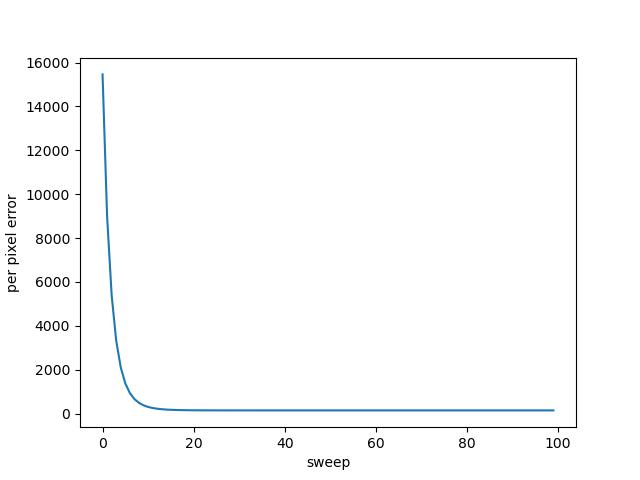
\includegraphics[width=\linewidth]{fig/loss/stone_big_loss.jpg}
        \caption{stone big}
    \end{subfigure}%
    \hfill%
    \begin{subfigure}[]{0.333\linewidth}
        \centering
        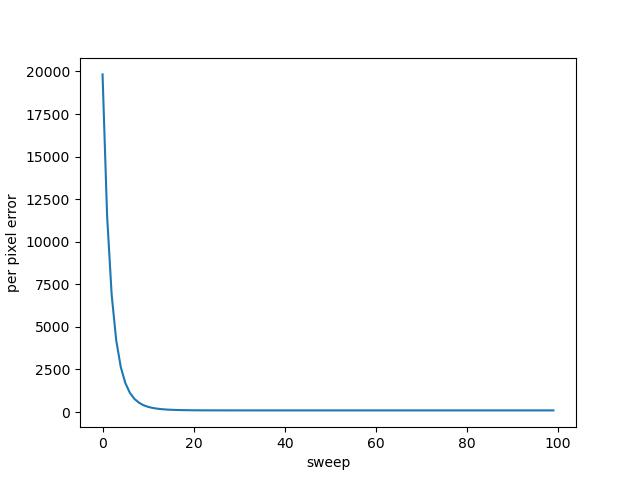
\includegraphics[width=\linewidth]{fig/loss/sce_big_loss.jpg}
        \caption{sce big}
    \end{subfigure}%
    \hfill%
    \begin{subfigure}[]{0.333\linewidth}
        \centering
        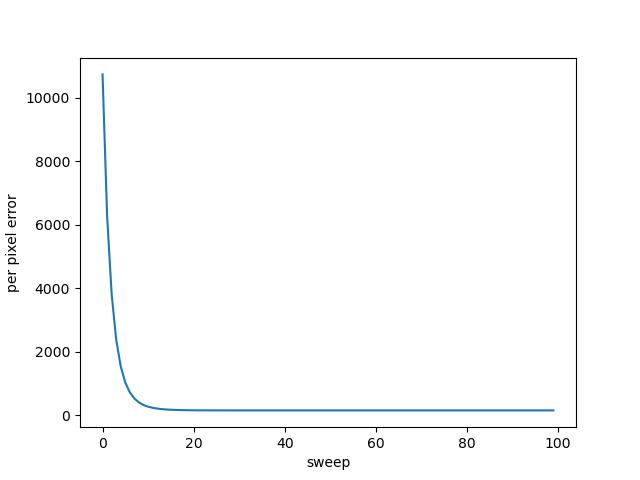
\includegraphics[width=\linewidth]{fig/loss/room_big_loss.jpg}
        \caption{room big}
    \end{subfigure}%
\end{figure}

\subsection{Restored Image}

\subsubsection{Gibbs Restoration}

\begin{figure}[ht!]
    \centering
    \hfill%
    \begin{subfigure}[]{0.333\linewidth}
        \centering
        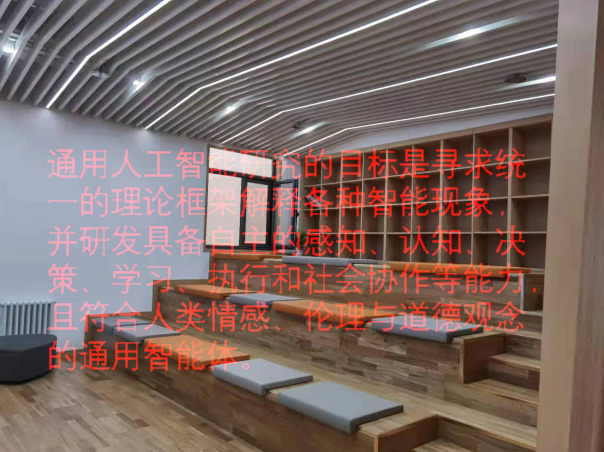
\includegraphics[width=\linewidth]{fig/restoration/room_big/L1/gibbs_0.jpg}
        \caption{room big L1 sweep 0}
    \end{subfigure}%
    \hfill%
    \begin{subfigure}[]{0.333\linewidth}
        \centering
        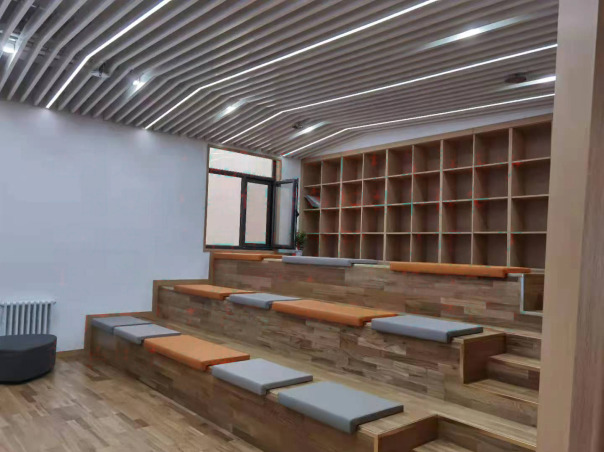
\includegraphics[width=\linewidth]{fig/restoration/room_big/L1/gibbs_10.jpg}
        \caption{room big L1 sweep 10}
    \end{subfigure}%
    \hfill%
    \begin{subfigure}[]{0.333\linewidth}
        \centering
        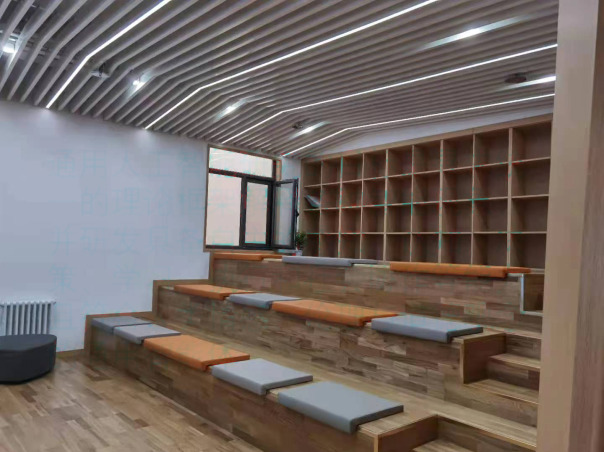
\includegraphics[width=\linewidth]{fig/restoration/room_big/L1/gibbs_99.jpg}
        \caption{room big L1 sweep 99}
    \end{subfigure}%
\end{figure}

\begin{figure}[ht!]
    \centering
    \hfill%
    \begin{subfigure}[]{0.333\linewidth}
        \centering
        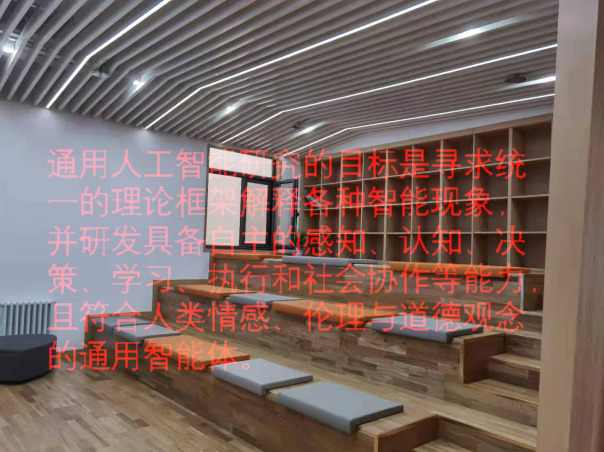
\includegraphics[width=\linewidth]{fig/restoration/room_big/L2/gibbs_0.jpg}
        \caption{room big L2 sweep 0}
    \end{subfigure}%
    \hfill%
    \begin{subfigure}[]{0.333\linewidth}
        \centering
        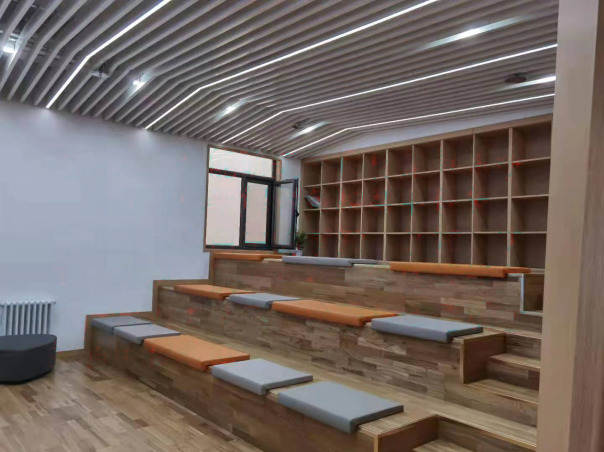
\includegraphics[width=\linewidth]{fig/restoration/room_big/L2/gibbs_10.jpg}
        \caption{room big L2 sweep 10}
    \end{subfigure}%
    \hfill%
    \begin{subfigure}[]{0.333\linewidth}
        \centering
        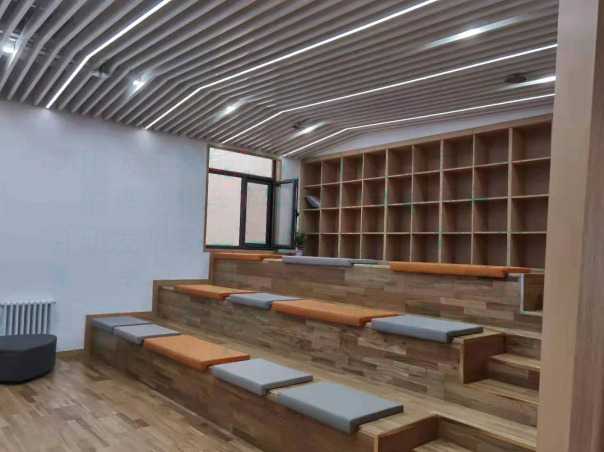
\includegraphics[width=\linewidth]{fig/restoration/room_big/L2/gibbs_99.jpg}
        \caption{room big L2 sweep 99}
    \end{subfigure}%
\end{figure}

\begin{figure}[ht!]
    \centering
    \hfill%
    \begin{subfigure}[]{0.333\linewidth}
        \centering
        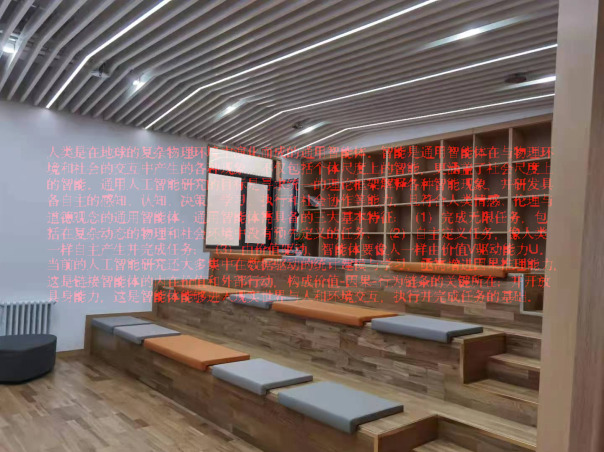
\includegraphics[width=\linewidth]{fig/restoration/room_small/L1/gibbs_0.jpg}
        \caption{room small L1 sweep 0}
    \end{subfigure}%
    \hfill%
    \begin{subfigure}[]{0.333\linewidth}
        \centering
        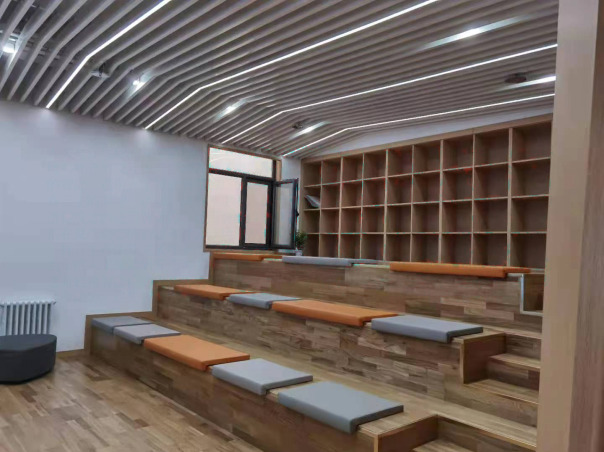
\includegraphics[width=\linewidth]{fig/restoration/room_small/L1/gibbs_10.jpg}
        \caption{room small L1 sweep 10}
    \end{subfigure}%
    \hfill%
    \begin{subfigure}[]{0.333\linewidth}
        \centering
        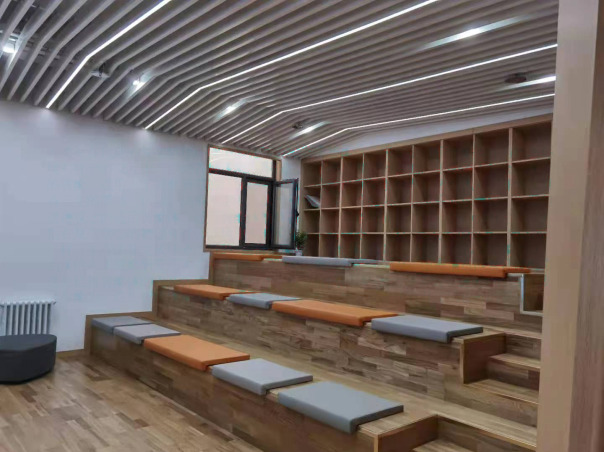
\includegraphics[width=\linewidth]{fig/restoration/room_small/L1/gibbs_99.jpg}
        \caption{room small L1 sweep 99}
    \end{subfigure}%
\end{figure}

\begin{figure}[ht!]
    \centering
    \hfill%
    \begin{subfigure}[]{0.333\linewidth}
        \centering
        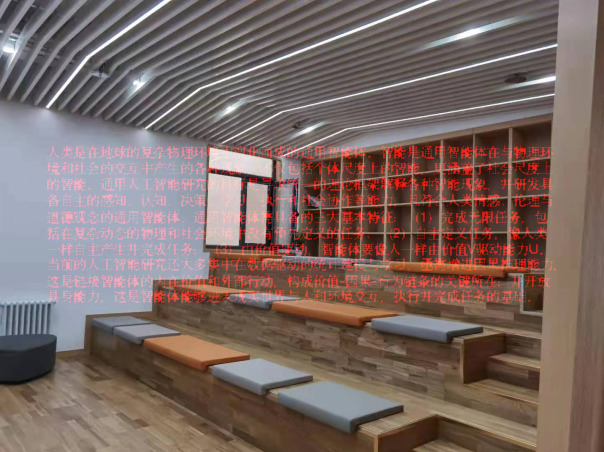
\includegraphics[width=\linewidth]{fig/restoration/room_small/L2/gibbs_0.jpg}
        \caption{room small L2 sweep 0}
    \end{subfigure}%
    \hfill%
    \begin{subfigure}[]{0.333\linewidth}
        \centering
        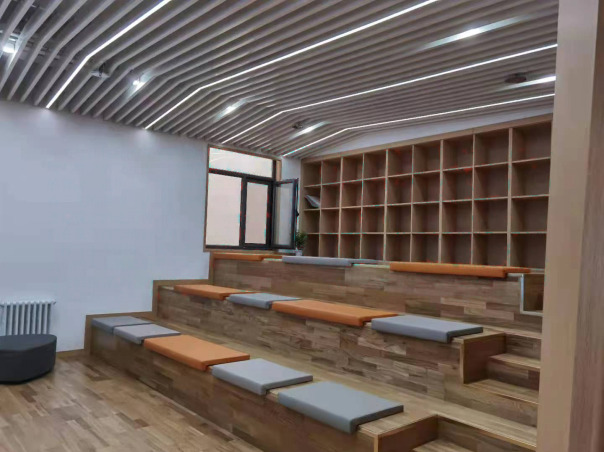
\includegraphics[width=\linewidth]{fig/restoration/room_small/L2/gibbs_10.jpg}
        \caption{room small L2 sweep 10}
    \end{subfigure}%
    \hfill%
    \begin{subfigure}[]{0.333\linewidth}
        \centering
        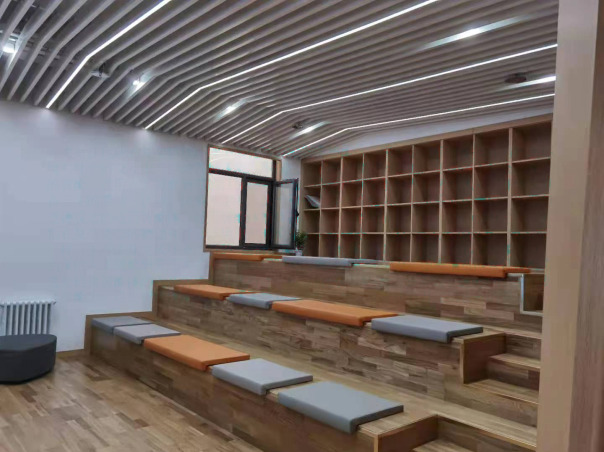
\includegraphics[width=\linewidth]{fig/restoration/room_small/L2/gibbs_99.jpg}
        \caption{room small L2 sweep 99}
    \end{subfigure}%
\end{figure}

\begin{figure}[ht!]
    \centering
    \hfill%
    \begin{subfigure}[]{0.333\linewidth}
        \centering
        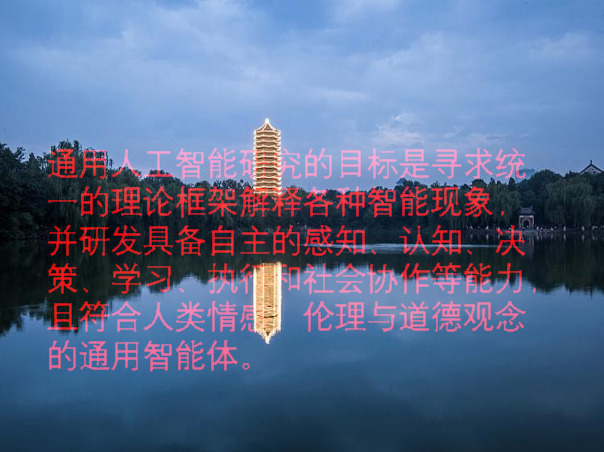
\includegraphics[width=\linewidth]{fig/restoration/sce_big/L1/gibbs_0.jpg}
        \caption{sce big L1 sweep 0}
    \end{subfigure}%
    \hfill%
    \begin{subfigure}[]{0.333\linewidth}
        \centering
        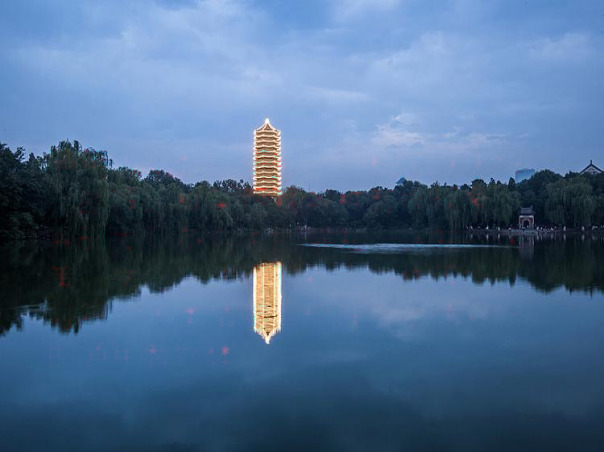
\includegraphics[width=\linewidth]{fig/restoration/sce_big/L1/gibbs_10.jpg}
        \caption{sce big L1 sweep 10}
    \end{subfigure}%
    \hfill%
    \begin{subfigure}[]{0.333\linewidth}
        \centering
        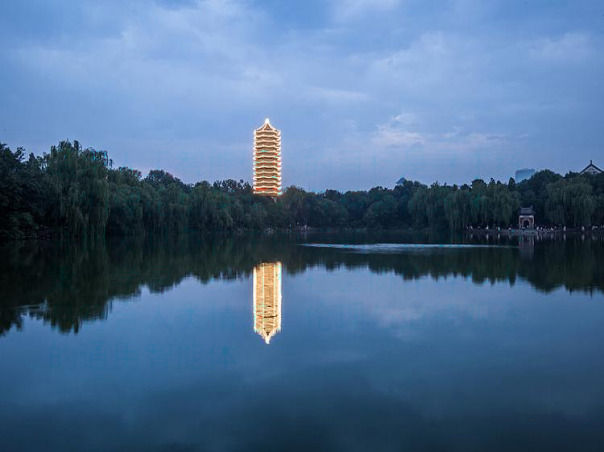
\includegraphics[width=\linewidth]{fig/restoration/sce_big/L1/gibbs_99.jpg}
        \caption{sce big L1 sweep 99}
    \end{subfigure}%
\end{figure}

\begin{figure}[ht!]
    \centering
    \hfill%
    \begin{subfigure}[]{0.333\linewidth}
        \centering
        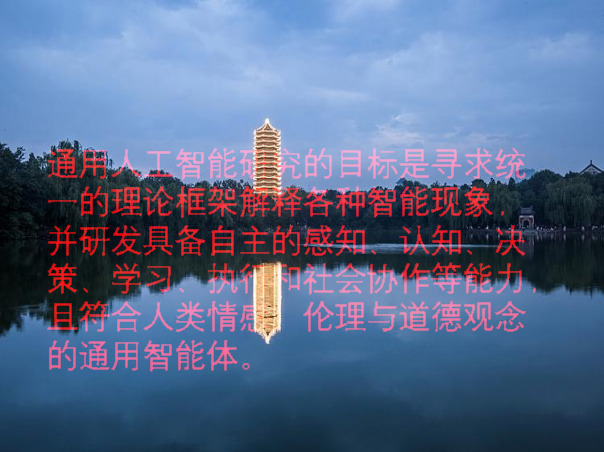
\includegraphics[width=\linewidth]{fig/restoration/sce_big/L2/gibbs_0.jpg}
        \caption{sce big L2 sweep 0}
    \end{subfigure}%
    \hfill%
    \begin{subfigure}[]{0.333\linewidth}
        \centering
        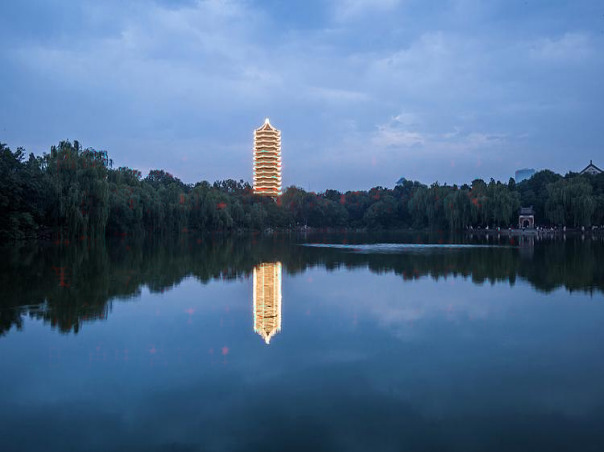
\includegraphics[width=\linewidth]{fig/restoration/sce_big/L2/gibbs_10.jpg}
        \caption{sce big L2 sweep 10}
    \end{subfigure}%
    \hfill%
    \begin{subfigure}[]{0.333\linewidth}
        \centering
        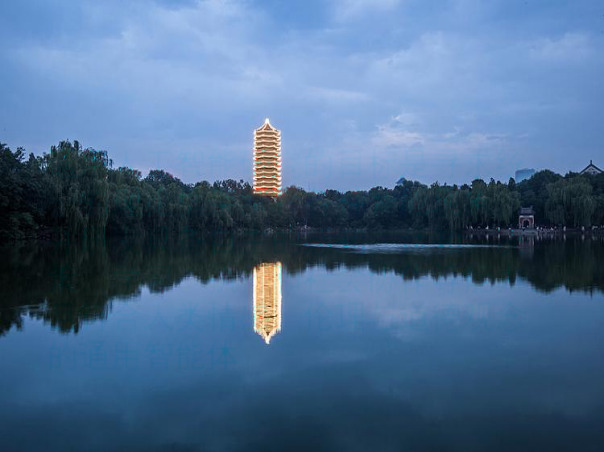
\includegraphics[width=\linewidth]{fig/restoration/sce_big/L2/gibbs_99.jpg}
        \caption{sce big L2 sweep 99}
    \end{subfigure}%
\end{figure}

\begin{figure}[ht!]
    \centering
    \hfill%
    \begin{subfigure}[]{0.333\linewidth}
        \centering
        \includegraphics[width=\linewidth]{fig/restoration/sce_small/L1/gibbs_0.jpg}
        \caption{sce small L1 sweep 0}
    \end{subfigure}%
    \hfill%
    \begin{subfigure}[]{0.333\linewidth}
        \centering
        \includegraphics[width=\linewidth]{fig/restoration/sce_small/L1/gibbs_10.jpg}
        \caption{sce small L1 sweep 10}
    \end{subfigure}%
    \hfill%
    \begin{subfigure}[]{0.333\linewidth}
        \centering
        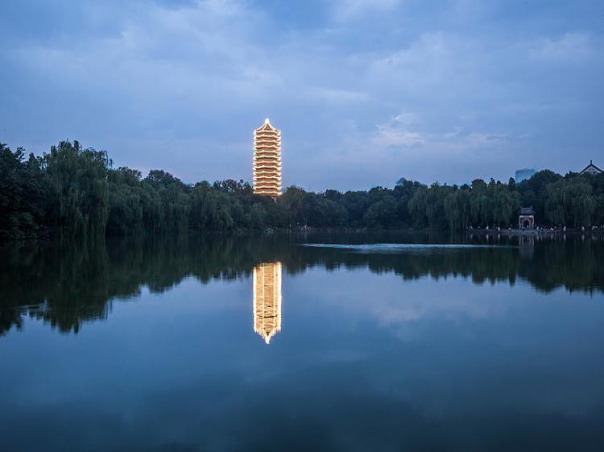
\includegraphics[width=\linewidth]{fig/restoration/sce_small/L1/gibbs_99.jpg}
        \caption{sce small L1 sweep 99}
    \end{subfigure}%
\end{figure}

\begin{figure}[ht!]
    \centering
    \hfill%
    \begin{subfigure}[]{0.333\linewidth}
        \centering
        \includegraphics[width=\linewidth]{fig/restoration/sce_small/L2/gibbs_0.jpg}
        \caption{sce small L2 sweep 0}
    \end{subfigure}%
    \hfill%
    \begin{subfigure}[]{0.333\linewidth}
        \centering
        \includegraphics[width=\linewidth]{fig/restoration/sce_small/L2/gibbs_10.jpg}
        \caption{sce small L2 sweep 10}
    \end{subfigure}%
    \hfill%
    \begin{subfigure}[]{0.333\linewidth}
        \centering
        \includegraphics[width=\linewidth]{fig/restoration/sce_small/L2/gibbs_99.jpg}
        \caption{sce small L2 sweep 99}
    \end{subfigure}%
\end{figure}

\begin{figure}[ht!]
    \centering
    \hfill%
    \begin{subfigure}[]{0.333\linewidth}
        \centering
        \includegraphics[width=\linewidth]{fig/restoration/stone_big/L1/gibbs_0.jpg}
        \caption{stone big L1 sweep 0}
    \end{subfigure}%
    \hfill%
    \begin{subfigure}[]{0.333\linewidth}
        \centering
        \includegraphics[width=\linewidth]{fig/restoration/stone_big/L1/gibbs_10.jpg}
        \caption{stone big L1 sweep 10}
    \end{subfigure}%
    \hfill%
    \begin{subfigure}[]{0.333\linewidth}
        \centering
        \includegraphics[width=\linewidth]{fig/restoration/stone_big/L1/gibbs_99.jpg}
        \caption{stone big L1 sweep 99}
    \end{subfigure}%
\end{figure}

\begin{figure}[ht!]
    \centering
    \hfill%
    \begin{subfigure}[]{0.333\linewidth}
        \centering
        \includegraphics[width=\linewidth]{fig/restoration/stone_big/L2/gibbs_0.jpg}
        \caption{stone big L2 sweep 0}
    \end{subfigure}%
    \hfill%
    \begin{subfigure}[]{0.333\linewidth}
        \centering
        \includegraphics[width=\linewidth]{fig/restoration/stone_big/L2/gibbs_10.jpg}
        \caption{stone big L2 sweep 10}
    \end{subfigure}%
    \hfill%
    \begin{subfigure}[]{0.333\linewidth}
        \centering
        \includegraphics[width=\linewidth]{fig/restoration/stone_big/L2/gibbs_99.jpg}
        \caption{stone big L2 sweep 99}
    \end{subfigure}%
\end{figure}

\begin{figure}[ht!]
    \centering
    \hfill%
    \begin{subfigure}[]{0.333\linewidth}
        \centering
        \includegraphics[width=\linewidth]{fig/restoration/stone_small/L1/gibbs_0.jpg}
        \caption{stone small L1 sweep 0}
    \end{subfigure}%
    \hfill%
    \begin{subfigure}[]{0.333\linewidth}
        \centering
        \includegraphics[width=\linewidth]{fig/restoration/stone_small/L1/gibbs_10.jpg}
        \caption{stone small L1 sweep 10}
    \end{subfigure}%
    \hfill%
    \begin{subfigure}[]{0.333\linewidth}
        \centering
        \includegraphics[width=\linewidth]{fig/restoration/stone_small/L1/gibbs_99.jpg}
        \caption{stone small L1 sweep 99}
    \end{subfigure}%
\end{figure}

\begin{figure}[ht!]
    \centering
    \hfill%
    \begin{subfigure}[]{0.333\linewidth}
        \centering
        \includegraphics[width=\linewidth]{fig/restoration/stone_small/L2/gibbs_0.jpg}
        \caption{stone small L2 sweep 0}
    \end{subfigure}%
    \hfill%
    \begin{subfigure}[]{0.333\linewidth}
        \centering
        \includegraphics[width=\linewidth]{fig/restoration/stone_small/L2/gibbs_10.jpg}
        \caption{stone small L2 sweep 10}
    \end{subfigure}%
    \hfill%
    \begin{subfigure}[]{0.333\linewidth}
        \centering
        \includegraphics[width=\linewidth]{fig/restoration/stone_small/L2/gibbs_99.jpg}
        \caption{stone small L2 sweep 99}
    \end{subfigure}%
\end{figure}

\subsubsection{PDE Restoration}

\begin{figure}[ht!]
    \centering
    \hfill%
    \begin{subfigure}[]{0.333\linewidth}
        \centering
        \includegraphics[width=\linewidth]{fig/restoration/room_big/pde_0.jpg}
        \caption{room big pde sweep 0}
    \end{subfigure}%
    \hfill%
    \begin{subfigure}[]{0.333\linewidth}
        \centering
        \includegraphics[width=\linewidth]{fig/restoration/room_big/pde_10.jpg}
        \caption{room big pde sweep 10}
    \end{subfigure}%
    \hfill%
    \begin{subfigure}[]{0.333\linewidth}
        \centering
        \includegraphics[width=\linewidth]{fig/restoration/room_big/pde_90.jpg}
        \caption{room big pde sweep 90}
    \end{subfigure}%
\end{figure}

\begin{figure}[ht!]
    \centering
    \hfill%
    \begin{subfigure}[]{0.333\linewidth}
        \centering
        \includegraphics[width=\linewidth]{fig/restoration/room_small/pde_0.jpg}
        \caption{room small pde sweep 0}
    \end{subfigure}%
    \hfill%
    \begin{subfigure}[]{0.333\linewidth}
        \centering
        \includegraphics[width=\linewidth]{fig/restoration/room_small/pde_10.jpg}
        \caption{room small pde sweep 10}
    \end{subfigure}%
    \hfill%
    \begin{subfigure}[]{0.333\linewidth}
        \centering
        \includegraphics[width=\linewidth]{fig/restoration/room_small/pde_90.jpg}
        \caption{room small pde sweep 90}
    \end{subfigure}%
\end{figure}

\begin{figure}[ht!]
    \centering
    \hfill%
    \begin{subfigure}[]{0.333\linewidth}
        \centering
        \includegraphics[width=\linewidth]{fig/restoration/sce_big/pde_0.jpg}
        \caption{sce big pde sweep 0}
    \end{subfigure}%
    \hfill%
    \begin{subfigure}[]{0.333\linewidth}
        \centering
        \includegraphics[width=\linewidth]{fig/restoration/sce_big/pde_10.jpg}
        \caption{sce big pde sweep 10}
    \end{subfigure}%
    \hfill%
    \begin{subfigure}[]{0.333\linewidth}
        \centering
        \includegraphics[width=\linewidth]{fig/restoration/sce_big/pde_90.jpg}
        \caption{sce big pde sweep 90}
    \end{subfigure}%
\end{figure}

\begin{figure}[ht!]
    \centering
    \hfill%
    \begin{subfigure}[]{0.333\linewidth}
        \centering
        \includegraphics[width=\linewidth]{fig/restoration/sce_small/pde_0.jpg}
        \caption{sce small pde sweep 0}
    \end{subfigure}%
    \hfill%
    \begin{subfigure}[]{0.333\linewidth}
        \centering
        \includegraphics[width=\linewidth]{fig/restoration/sce_small/pde_10.jpg}
        \caption{sce small pde sweep 10}
    \end{subfigure}%
    \hfill%
    \begin{subfigure}[]{0.333\linewidth}
        \centering
        \includegraphics[width=\linewidth]{fig/restoration/sce_small/pde_90.jpg}
        \caption{sce small pde sweep 90}
    \end{subfigure}%
\end{figure}

\begin{figure}[ht!]
    \centering
    \hfill%
    \begin{subfigure}[]{0.333\linewidth}
        \centering
        \includegraphics[width=\linewidth]{fig/restoration/stone_big/pde_0.jpg}
        \caption{stone big pde sweep 0}
    \end{subfigure}%
    \hfill%
    \begin{subfigure}[]{0.333\linewidth}
        \centering
        \includegraphics[width=\linewidth]{fig/restoration/stone_big/pde_10.jpg}
        \caption{stone big pde sweep 10}
    \end{subfigure}%
    \hfill%
    \begin{subfigure}[]{0.333\linewidth}
        \centering
        \includegraphics[width=\linewidth]{fig/restoration/stone_big/pde_90.jpg}
        \caption{stone big pde sweep 90}
    \end{subfigure}%
\end{figure}

\begin{figure}[ht!]
    \centering
    \hfill%
    \begin{subfigure}[]{0.333\linewidth}
        \centering
        \includegraphics[width=\linewidth]{fig/restoration/stone_small/pde_0.jpg}
        \caption{stone small pde sweep 0}
    \end{subfigure}%
    \hfill%
    \begin{subfigure}[]{0.333\linewidth}
        \centering
        \includegraphics[width=\linewidth]{fig/restoration/stone_small/pde_10.jpg}
        \caption{stone small pde sweep 10}
    \end{subfigure}%
    \hfill%
    \begin{subfigure}[]{0.333\linewidth}
        \centering
        \includegraphics[width=\linewidth]{fig/restoration/stone_small/pde_90.jpg}
        \caption{stone small pde sweep 90}
    \end{subfigure}%
\end{figure}

\subsection{Original Pictures}

\begin{figure}[ht!]
    \centering
    \hfill%
    \begin{subfigure}[]{0.333\linewidth}
        \centering
        \includegraphics[width=\linewidth]{fig/room.jpg}
        \caption{original room}
    \end{subfigure}%
    \hfill%
    \begin{subfigure}[]{0.333\linewidth}
        \centering
        \includegraphics[width=\linewidth]{fig/sce.jpg}
        \caption{original sce}
    \end{subfigure}%
    \hfill%
    \begin{subfigure}[]{0.333\linewidth}
        \centering
        \includegraphics[width=\linewidth]{fig/stone.jpg}
        \caption{original stone}
    \end{subfigure}%
\end{figure}

\end{document}